\documentclass[tikz, margin=1in]{standalone}

\usetikzlibrary{calc, arrows.meta, bending}

\definecolor{mygray}{HTML}{aaaaaa}

\begin{document}
    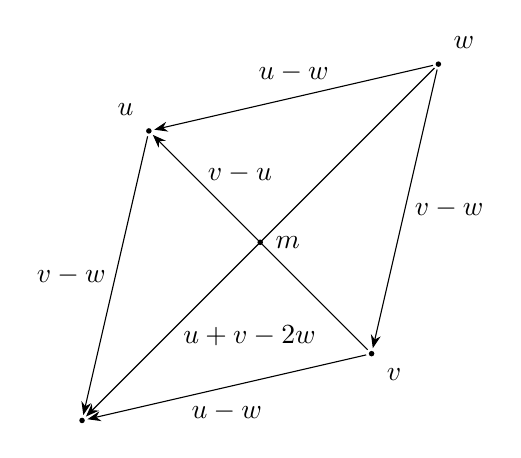
\begin{tikzpicture}[ 
            % color=mygray,  
            point/.style={radius=1pt},
            vec/.style={arrows=-Stealth, shorten >=2pt, shorten <=2pt}            
        ]

        \coordinate (u) at ($(2,1) + (135:2)$);
        \coordinate (v) at ($(2,1) + (315:2)$);
        \coordinate (m) at ($(u)!0.5!(v)$);


        \path let \p{uv} = ($(v)-(u)$),
                  \p{uv'} = ($0.8*(\p{uv})$),
                  \p{uvOrtho} = (-\y{uv'}, \x{uv'}) 
              in coordinate (w) at ($(m)+(\p{uvOrtho})$)
                 coordinate (w*) at ($(m)-(\p{uvOrtho})$);

        \fill (u) circle[point] node[above left=2pt] {\(u\)};
        \fill (v) circle[point] node[below right=2pt] {\(v\)};
        \fill (w) circle[point] node[above right=2pt] {\(w\)};
        \fill (m) circle[point] node[right=2pt] {\(m\)};
        \fill (w*) circle[point];

        \draw[vec] (w) to node[above=2pt] {\(u-w\)} (u);
        \draw[vec] (w) to node[right=0pt] {\(v-w\)} (v);
        \draw[vec] (v) to node[below=2pt] {\(u-w\)} (w*);
        \draw[vec] (u) to node[left=0pt] {\(v-w\)} (w*);
        \draw[vec] (w) to node[pos=.725, below right=0pt, inner sep=1pt] {\(u+v-2w\)} (w*);
        \draw[vec] (v) to node[pos=.75, above right=0pt, inner sep=1pt] {\(v-u\)} (u);
    \end{tikzpicture}
\end{document}